%https://www.slideshare.net/maheshkha/cuda-tutorial (Memory space)
% https://www.slideshare.net/Hanibei/cuda-introduction - Kernel memory access
% https://www.microway.com/hpc-tech-tips/gpu-memory-types-performance-comparison/
%Husk at tjekke Shane Cook Hardware architecture afsnittet her.
%TODO Understanding NVIDIA GPGPU Hardware
%TODO Update to newest ( and consider all cahces)

As presented through the earlier sections, the GPU hardware architecture contains multiple types of memories \& caches.
As these individual types vary in size, speed, accessibility \& lifetime one must know their context and features.
This section provides a understanding of these different memory types, but as the other components within the architecture, these changes as well depending on the architecture version.
Therefore, the memory model presented in this section also is a conceptual model, with the focus of providing general understanding.
First the memory types are presented in \cref{sec-mem-types}, and hereafter the caches in \cref{sec-cac-types}.

\subsubsection{Memory types}
\label{sec-mem-types}
\textbf{Register File -} As presented in \cref{sec-hw-streaming-processors}, the Register Files are located in the SMs and used by SPs as registers.
Due to the SIMT execution model, a large number of threads are run on a SP at a given time.
This results in a high demand for a large volume of registers, which due to its large size is implemented by SRAMs \cite{Li2016}.
As described in \cref{sec-hw-warps-threads}, the Register File is shared between the different warps running on a SM.
To increase the allocation capabilities in this sharing, the registers within the Register File are not dedicated to specific cores, but instead potentially shareable by each thread.
On the execution of threads, the SM assigns registers to it, which are bound to the thread until its lifetime ends.
In this access binding, no other thread can access the register for read or write operations.
For most architecture types, the Register Files speed matches the clock cycle of the SPs, allowing for zero clock cycles per instruction to access a given register.
For that reason, the Register File is the fastest memory accessible in the GPU memory model.
\\\\
\textbf{Local Memory -} The Local Memory is actually a portion of the Global Memory.
It is therefore not as such a physical memory space but only a partition.
Differing from the Global Memory, its accessibility scope is per-thread just like the Register File.
It is generally used for \textit{register spilling}, meaning that if the amount of registers available in the Register File is insufficient for the amount of variables in the application, they are instead saved in the Local Memory.
Depending on the hardware architecture, the Local Memory is either cached by both by L1 and L2 Cache or only the L2 Cache.
The need of Local Memory due to register spilling reduces the performance greatly.
As illustrated on \cref{fig:hw-memory-schematic}, the Register File is the fastest memory accessible in the GPU, whereas the Local Memory if not cached matches the speed of the Global Memory. 
Now, with register spilling, the register speed is in best case reduced to the speed of the L1 and L2 Caches.
In the case of what is known as a cache miss, meaning that the data is unaccessible through the cache, the value must be fetched from the off-chip Global Memory, greatly reducing the speed.
The lifetime of the Local Memory matches the Register File, meaning that once the thread which uses a part of the memory terminates, the memory is freed.
\begin{figure}[H]
	\centering
	\fbox{
		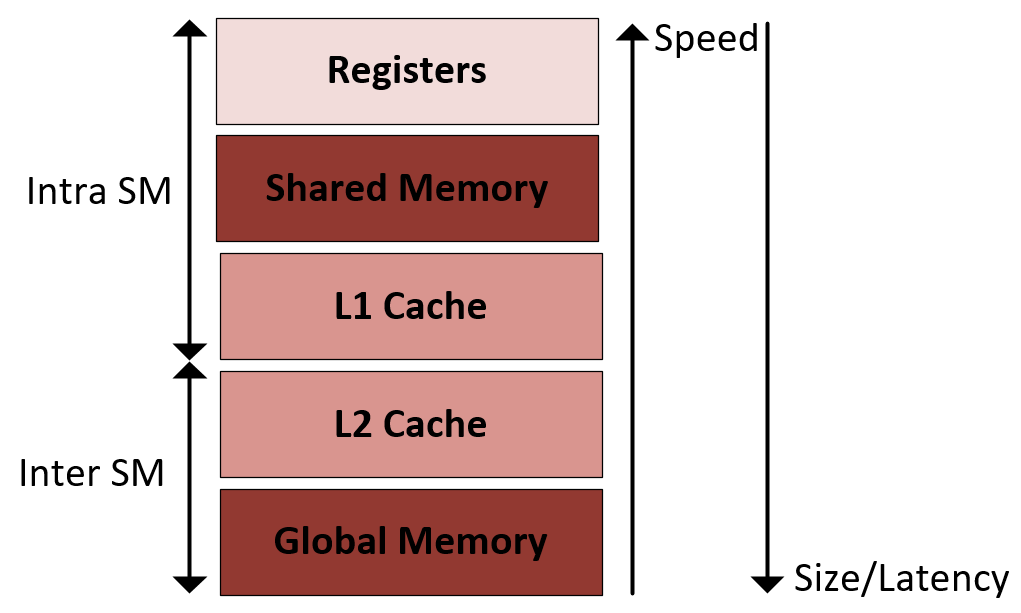
\includegraphics[width=0.6\textwidth]{figs/hw/hw-memory-schematic}}
	\caption{GPU memory schematic}
	\label{fig:hw-memory-schematic}
\end{figure}
\noindent \textbf{Shared Memory -} Different from the Local and Global Memory, the Shared Memory is located on the SM chip.
Its access scope, which is per Thread Block as illustrated on \cref{fig:hw-memory-model}, allows for it to be used for data exchange  between the threads located within the given block.
The Shared Memory is partitioned into a series of banks, which are handled by a bus, allowing for very fast access like the Register File, which allows for a high bandwidth and low access latency \cite{Li2016}.
The fastest possible configuration requires each bank to be served by only a single thread, allowing for parallel accessing of every bank.
If multiple threads are to share the same bank, accessing is serialized, which is also defined as \textit{bank conflicting} \cite{Maitre2013}.
As presented in \cref{ch-opti-intro}, various optimizations should be kept in mind when working on the GPU, this includes using the Shared Memory over the Global or Local Memory when possible.
\\\\
\textbf{Global Memory -} The Global Memory is also known as \textit{Device Memory}, \textit{GPU off-chip Memory} or \textit{GPU Main Memory}.
Different from the previously presented memory types, the data stored that is stored in the Global Memory is visible to all threads within the GPU application, as well as the CPU \textit{Host}. 
In addition, the lifetime  of the data lasts for the duration of the host allocation.
The Global Memory is used most frequently of all the memory types.
Because of this, its throughput often dictates the final achievable performance of the GPU.
To increase this performance, optimization aspects of accessing the Global Memory is presented in \cref{sec-opti-memory}.
The Global Memory is commonly implemented in DRAM memory and partitioned into three additional memories, namely Local, Texture and Constant memory.
\\\\
\begin{figure}[H]
	\centering
	\fbox{
		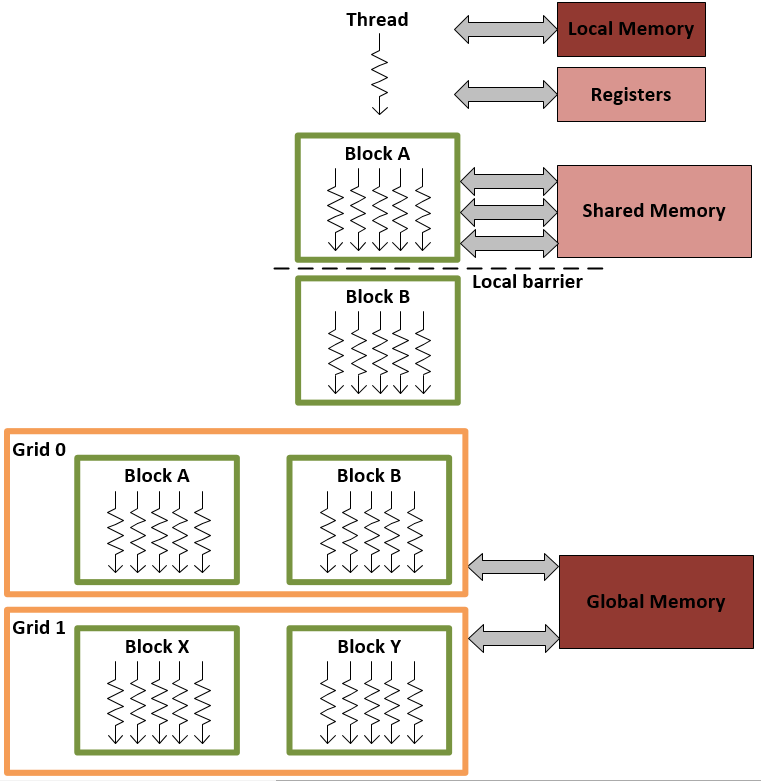
\includegraphics[width=0.93\textwidth]{figs/hw/hw-memory-model}}
	\caption{GPU memory access scopes}
	\label{fig:hw-memory-model}
\end{figure}
\noindent \textbf{Texture Memory/Cache -} As the Local and Constant Memory, the Texture memory is allocated in the Global Memory area.
The Texture Memory is cached by the Texture Cache, which is specially optimized for 2D spatial locality. Therefore, threads from a warp can gain extra performance when they access nearby addresses in 2D space \cite{Li2016}.
\\\\
\textbf{Constant Memory/Cache -} The Constant Memory is also allocated in the Global Memory.
It is used for storing of data which is kept constant during execution of \textit{kernels}.
The Constant Memory is cached by its own Constant Cache, and therefore it does not use the L1 or L2 cache.

\subsubsection{Cache types}
\label{sec-cac-types}
\textbf{L1 Cache -} The L1 Cache, which is also known as the \textit{Data-Cache}, is located within each SM, where its primary job is to allow for faster Global Memory access.
Depending on the architecture version, the L1 Cache can either share the same storage as the Shared Memory, or have its own memory space.
It is used to perform reads/write operations on the Local Memory and read only operation on the Global Memory.
In addition it is used in case of register spills of the Register File as described earlier.
The L1 Cache is the fastest available cache, but limited in its size, as it is located locally on each SM.
\\\\
\textbf{L2 Cache -} The L2 Cache is a device-wide cache, used to access Global or Local Memory data, both through read and write operations.
As it is globally placed in between the different SMs, it can be used to share data across the different SMs using the Interconnection Network presented in \cref{sec-hw-gpu-arhchitecture}.
Compared to accessing the Global Memory from a SM, using the L2 Cache is an order of magnitude faster \cite{Cook2008}.
Compared to the L1 Cache, the L2 cache is slower but much larger.
\\\\
\Cref{alg-gpu-mem} accumulates the main features presented above for the different Memory types, and links them with their available Cache types.

\begin{table}[]
	\begin{tabular}{|l|c|c|c|c|c|}
		\hline
		\textbf{Memory}          & \textbf{On/Off Chip(SM)} & \textbf{Cached} & \textbf{Access} & \textbf{Scope} & \textbf{Lifetime} \\ \hline
		\textbf{Register File}  & On                   & N/A             & Read/Write      & Per-Thread     & Thread            \\ \hline
		\textbf{Local Memory}    & Off                  & L1/L2           & Read/Write      & Per-Thread     & Thread            \\ \hline
		\textbf{Shared Memory}   & On                   & N/A             & Read/Write      & Thread Block   & Thread Block      \\ \hline
		\textbf{Global Memory}   & Off                  & L1/L2           & Read/Write      & GPU+CPU        & Host Allocation   \\ \hline
		\textbf{Constant Memory} & Off                  & Constant Cache  & Read Only       & GPU+CPU        & Host Allocation   \\ \hline
		\textbf{Texture Memory}  & Off                  & Texture Cache   & Read Only       & GPU+CPU        & Host Allocation   \\ \hline
	\end{tabular}
	\centering
	\captionof{table}{GPU Memory Features \cite{Li2016}}
	\label{alg-gpu-mem}
\end{table}

